\chapter{Studi Literatur}


%---------------------------------------------------------
\section{Hypertext Transfer Protocol (HTTP)}
%---------------------------------------------------------
HTTP merupakan sebuah protokol yang digunakan oleh aplikasi berbasis web dalam melakukan komunikasi antara \textit{client} / \textit{web browser} dan \textit{server} / \textit{web server} \citep{kurose2013computer}. Protokol ini merupakan protokol standar yang didefinisikan dalam RFC1945 dan RFC2616 oleh Internet Engineering Task Force (IETF) dalam mengatur mekanisme \textit{request} dan \textit{response} antara \textit{web browser} dengan \textit{web server}. Secara sederhana, protokol ini mengatur tentang bagaimana \textit{web browser} meminta sebuah halaman web kepada \textit{web server} untuk kemudian ditampilkan kepada pengguna.

\begin{figure}
    \centering
    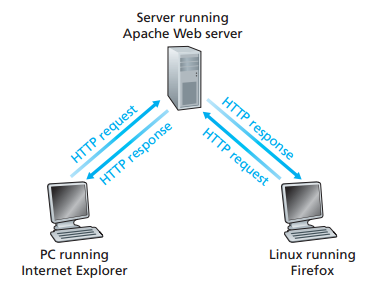
\includegraphics[width=0.6\textwidth]{img/http-behaviour.png}
    \caption{HTTP \textit{request} dan \textit{response}}
    \label{fig:httpBehaviour}
\end{figure}
\vspace{-0.8cm}
\begin{center}
{\small Sumber gambar: \citep{kurose2013computer}}
\end{center}

Seperti yang terlihat pada Gambar \ref{fig:httpBehaviour} diatas, komunikasi antara \textit{web browser} dengan \textit{web server} terjadi secara dua arah yaitu HTTP \textit{request} dan HTTP \textit{response}. HTTP \textit{request} adalah sebuah protokol yang digunakan oleh \textit{web browser} dalam meminta halaman web kepada \textit{web server} sedangkan HTTP \textit{response} adalah protokol yang digunakan oleh \textit{web server} dalam mengirimkan halaman web kepada \textit{web browser}. Dengan menggunkan mekanisme ini, pada saat pengguna aplikasi mengetikkan alamat \texttt{http://www.cs.ui.ac.id/index.php} pada \textit{web browser} yang digunakan, selanjutnya \textit{web browser} tersebut akan mengirimkan sebuah HTTP \textit{request} kepada \textit{web server} yang beralamat di \texttt{www.cs.ui.ac.id} untuk meminta sebuah halaman web bernama \texttt{index.php}. Setelah \textit{web server} menerima HTTP \textit{request} tersebut dan mencarikan halaman web yang diinginkan, selanjutnya \textit{web server} akan mengirimkan halaman web itu dengan menggunakan HTTP \textit{response} untuk kemudian ditampilkan kepada pengguna melalui \textit{web browser} yang digunakan.\\

Berikut ini adalah format dari HTTP \textit{message} sesuai dengan standar RFC2616 (HTTP/1.1) yang dibuat oleh \cite{webrfc2616}:

\begin{lstlisting}[
language=TeX,
caption=Format HTTP \textit{message} pada RFC2616,
label={lst:httpFormat}
]
HTTP-message      = Request | Response     ; HTTP/1.1 messages
generic-message   = start-line
                    *(message-header CRLF)
                    CRLF
                    [ message-body ]
start-line        = Request-Line | Status-Line

message-header    = field-name ":" [ field-value ]
field-name        = token
field-value       = *( field-content | LWS )
field-content     = <the OCTETs making up the field-value
                    and consisting of either *TEXT or combinations
                    of token, separators, and quoted-string>
                    
message-body      = entity-body
                    | <entity-body encoded as per Transfer-Encoding>

\end{lstlisting}

Seperti yang terlihat pada Kode \ref{lst:httpFormat} diatas, setiap pesan HTTP baik \textit{request} ataupun \textit{response} memiliki format yang sama yaitu terdiri dari \texttt{start-line}, \texttt{message-header} dan \texttt{message-body}. \texttt{Start-line} merupakan baris pembukan pada setiap pesan HTTP yang menandakan bahwa pesan tersebut merupakan pesan HTTP seperti misalnya \texttt{POST /product/details.abs HTTP/1.1} sedangkan \textit{message-header} merupakan kepala pesan yang berisi informasi terkait pesan tersebut seperti misalnya \texttt{Host}, \texttt{Connection}, \texttt{Content-Length}, \texttt{User-Agent} dan \texttt{Content-Type}. Terakhir adalah \texttt{message-body} yang merupakan isi dari pesan HTTP yang dikirimkan seperti misalnya data yang diberikan oleh pengguna web melalui \textit{form} HTML seperti misalnya \texttt{product\_sku=00188\&product\_name=FMSE+Dining+Set}.

%---------------------------------------------------------
\section{Model View Controller}
%---------------------------------------------------------

\textit{Model-View-Controller} (MVC) atau yang biasa juga dikenal dengan sebutan \textit{Presentation-Abstraction-Control} (PAC) merupakan salah satu pendekatan dalam proses pengembangan perangkat lunak yang ditujukan untuk melakukan pemisahan antara logika aplikasi, data, dan presentasi. Konsep ini dibangun atas kesadaran bahwa sebuah model domain aplikasi yang sama dapat disajikan dan diperlakukan secara berbeda tergantung dari kebutuhan si pengguna aplikasi. Dengan menggunakan pendekatan ini, seorang pengembang perangkat lunak dapat berfokus pada satu bagian saja tanpa harus mengkhawatirkan akan terkena dampak perubahan ataupun memberikan perubahan ke bagian aplikasi lainnya.

\subsection{Sejarah Singkat MVC}

Konsep MVC diterapkan pertama kalinya oleh Alan Kay, Dan Ingalls, dan Adele Goldberg pada tahun 1980 ketika mereka merancang bahasa pemrograman smalltalk-80 di Xerox PARC Learning Research Group (LRG) \citep{krasner1988desc}. bahasa pemrograman ini didesain dan dikembangkan dengan menggunakan strategi yang merepresentasikan informasi, tampilan, dan kontrol pada lingkungan pemrogramannya. Strategi ini digunakan dengan tujuan (1) untuk membuat kumpulan komponen sistem spesial yang dibutuhkan dalam mendukung proses pengembangan perangkat lunak yang interaktif serta (2) menyediakan kumpulan komponen sistem umum yang dapat membantu pengembang dalam menciptakan aplikasi grafis yang interaktif dengan mudah \citep{krasner1988desc}. Strategi dan tujuan tersebut dibuat dalam rangka menjawab isu utama dalam pengembangan perangkat lunak yaitu terkait pemanfaatan kembali komponen yang telah dibuat (\textit{reusability}) dan kemudahan dalam menggabungkan setiap komponen aplikasi (\textit{plugability}). \\

Belajar dari pengalamannya dalam mengembangkan smalltalk-76, para pengembang smalltalk-80 menemukan bahwa untuk mencapai sebuah modularitas yang tinggi diperlukan adanya tiga buah pemisahan fokus dalam pengembangan aplikasi. Tiga buah pemisahan fokus tersebut antara lain adalah (1) memisahkan setiap komponen yang merepresentasikan model domain aplikasi dengan (2) cara yang digunakan untuk merepresentasikan model tersebut ke pengguna aplikasi dan (3) cara yang digunakan oleh pengguna dalam berinteraksi dengan model tersebut. Tiga buah pemisahan tersebut dapat terangkum dalam sebuah konsep yang disebut dengan \textit{Model-View-Controller} (MVC).

\subsection{Karakteristik Komponen MVC}

Penggunaan pola MVC dalam pengembangan perangkat lunak ditujukan untuk memisahkan fokus pengemabangan kedalam tiga buah komponen aplikasi yaitu data, presentasi dan proses bisnis. Dalam proses pengembangan perangkat lunak, setiap kode yang dibuat memiliki karakteristik khusus yang dapat dibedakan berdasarkan fungsinya apakah kode tersebut sebagai data, presentasi atau proses bisnis. Berdasarkan pemaparan yang diberikan oleh \cite{krasner1988desc}, \cite{leff2001web} dan \cite{burbeck1992applications}, terdapat beberapa karakteristik yang dapat digunakan untuk membedakan komponen-komponen MVC tersebut sesuai dengan fungsinya. Karakteristik-karakteristik tersebut antara lain adalah:

\begin{itemize}
    \item \textbf{Model} merupakan komponen aplikasi yang mengandung implementasi dari \textit{domain-spesific entity} dari aplikasi yang dibuat. komponen ini dapat hanya berupa sebuah integer untuk menghitung \textit{counter} atau berupa objek yang kompleks dengan banyak atribut didalamnya. Selain itu, komponen ini harus dapat mengelola  \textit{behaviour} dari data dengan cara menyediakan mekanisme yang dapat digunakan untuk mengetahui dan mengubah \textit{state} dari data tersebut.
    \item \textbf{View} merupakan komponen yang menangani seluruh permasalahan yang berkaitan dengan grafis. Secara umum, komponen ini merupakan komponen yang bertanggung jawab dalam menampilkan data sesuai dengan keinginan pengguna aplikasi baik dalam bentuk grafis ataupun tekstual.
    \item \textbf{Controller} merupakan komponen aplikasi yang bertanggung jawab dalam menjembatani komponen Model dan View. Secara umum, komponen ini memiliki kemampuan untuk menerima \textit{input} dari pengguna aplikasi dan memprosesnya sesuai dengan proses bisnis yang telah dibuat.
\end{itemize}

\subsection{Penerapan MVC dalam Pengembangan Aplikasi Web}
Aplikasi web merupakan aplikasi yang tergolong interaktif karena aplikasi jenis ini banyak memiliki elemen-elemen yang dapat digunakan untuk berinteraksi dengan penggunannya. Sebagai contoh, dalam sebuah halaman situs web tentunya kita akan menemukan banyak tombol, gambar, tautan, dan kotak isian yang dapat kita gunakan untuk berinteraksi dengan situs web tersebut. Untuk sebuah aplikasi yang tergolong interaktif, adanya pemisahan antara logika aplikasi, data, dan presentasi tentunya akan dapat meningkatkan fleksibilitas aplikasi tersebut dari segi pengembangan. \\

Pada dasarnya, arsitektur apliksi berbasis web terbagi menjadi dua bagian yaitu \textit{client} dan \textit{server}. Dengan arsitektur yang seperti ini, para pengembang aplikasi tidak dapat menentukan dengan jelas bagaimana bentuk partisi yang harus dibuat untuk aplikasi tersebut. Sebagai contoh, dengan adanya pembagian antara \textit{client} dan \textit{server}, para pengembang aplikasi harus menentukan dimanakah komponen \textit{view} akan dibentuk? Apakah komponen ini akan dibentuk di tingkat \textit{client} ataukah di tingkat \textit{server}. Begitupun dengan komponen \textit{Model} dan \textit{Controller
}-nya. Apakah komponen-komponen tersebut akan akan dibuat di tingkat \textit{client}, \textit{server}, atau keduanya? Pada akhirnya, keputusan dalam menentukan skema partisi yang dipakai akan sangat bergantung pada teknologi yang digunakan \citep{leff2001web}. \\

Permasalahan terkait pemisahan antara \textit{client} dan \textit{server} pada aplikasi berbasis web menjadikan penerapan MVC lebih sulit. Proses penerapan MVC akan dapat berhasil apabila (1) para pengembang aplikasi sudah mengetahui bagaimana skema partisi yang akan diterapkan serta (2) teknologi dan infrastruktur yang ada \textit{compatible} dengan skema partisi yang diterapkan. Oleh karena itu, perlu adanya sebuah pendekatan yang dapat digunakan oleh para pengembang untuk memastikan dua hal tersebut.

%---------------------------------------------------------
\section{Software Product Line Engineering (SPLE)}
%---------------------------------------------------------

\textit{Software Product Line Engineering} (SPLE) merupakan sebuah paradigma yang digunakan dalam proses pengembangan perangkat lunak dengan menggunakan prinsip \textit{platform} dan \textit{mass customisation} \citep[p.~14]{pohl2005software}. Dalam industri perangkat lunak, istilah \textit{platform} atau \textit{software platform} biasa diartikan sebagai sebuah sistem komputer (misal: prosesor atau kombinasi antara perangkat keras dengan sistem operasi) yang menyebabkan dapat berjalannya sebuah program komputer. Sedangkan dalam konteks SPLE, yang dimaksud dengan \textit{platform} adalah sebuah subsistem dan \textit{interface} yang membentuk sebuah struktur umum dimana nantinya sebuah produk turunan dapat dikembangkan dan diproduksi secara efisien \citep[p.~15]{pohl2005software}. \\

Dalam paradigma SPLE, proses pengembangan perangkat lunak dibagi menjadi dua bagian yaitu \textit{Domain Engineering} dan \textit{Application Engineering} \citep[p.~21]{pohl2005software}. \textit{Domain Engineering} adalah sebuah proses dalam SPLE dimana pada tahap ini seluruh \textit{commonality} dan \textit{variability} dari SPL didefinisikan dan direalisikan. Sedangkan tahap \textit{Application Engineering} adalah sebuah proses dimana aplikasi dari SPL dibuat dengan cara memanfaatkan \textit{domain artifact} yang telah dibuat pada tahap sebelumnya dan mengeksploitasi \textit{variability} yang ada di dalam SPL tersebut \cite{metzger2007variability}. Tahapan-tahapan proses dalam SPLE ini biasa disebut dengan istilah \textit{SPLE Framework} seperti yang terlihat pada Gambar \ref{fig:spleFramework} dibawah ini. \\

\begin{figure}
    \centering
    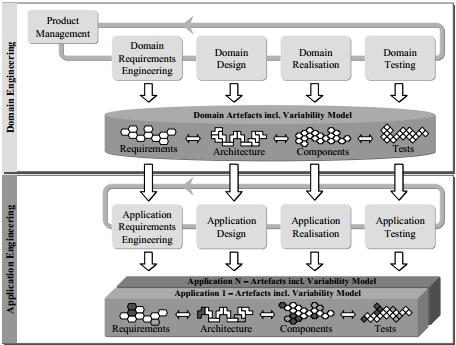
\includegraphics[width=0.8\textwidth]
        {img/sple-process.png}
    \caption{SPLE Framework}
    \label{fig:spleFramework}
\end{figure}
\vspace{-0.8cm}
\begin{center}
{\small Sumber gambar: \citep{pohl2005software}}
\end{center}

Seperti yang telah disebutkan pada paragraf sebelumnya, dalam sebuah paradigma SPLE dikenal dua buah istilah yang bernama \textit{commonality} (\textit{product commonality}) dan \textit{variability} (\textit{product line variability}). \textit{product Commonality} merupakan sebuah property yang digunakan secara bersama-sama pada setiap varian dalam \textit{SPL} sedangkan \textit{product line variability} adalah tingkat perbedaan dari setiap produk perangkat lunak yang dihasilkan dalam proses SPLE seperti misalnya perbedaan dalam hal fitur, \textit{functional requirement} dan kualitas dari perangkat lunak yang dihasilkan \cite{metzger2014software}.

%---------------------------------------------------------
\section{Abstract Behavioural Spesification (ABS)}
%---------------------------------------------------------

Abstract Behavioural Specification Language (ABS) merupakan sebuah bahasa pemodelan yang dibuat oleh konsorsium uni eropa di bawah proyek bernama \textit{Highly Adaptable and Trustworthy Software using Formal Method} (HATS). Tujuan dari proyek HATS dalam menciptakan ABS adalah untuk menciptakan sebuah pendekatan yang \textit{model-centric} dalam melakukan proses perancangan, implementasi dan verifikasi dari sebuah sistem yang \textit{highly-configurable} \citep{clarke2012variability}. Pada dasarnya ABS dibagi kedalam beberapa layer yang diantaranya adalah \textit{functional abstraction} (kuning), \textit{OO-Imperative layer} (hijau), \textit{Concurency Model} (biru) dan \textit{ABS Core} (merah jambu, lihat Gambar \ref{fig:absLayer}). \\

\begin{figure}
    \centering
    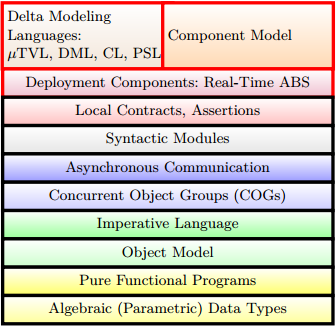
\includegraphics[width=0.6\textwidth]
        {img/abs-layers.png}
    \caption{ABS Layer}
    \label{fig:absLayer}
\end{figure}
\vspace{-0.8cm}
\begin{center}
{\small Sumber gambar: \citep{hahnle2013hats}}
\end{center}

Sebagai sebuah bahasa pemrograman \textit{imperative} yang menganut konsep \textit{Object Oriented}, secara umum ABS memiliki sintaks yang sama dengan bahasa pemrograman JAVA (walaupun lebih sederhana). Salah satu perbedaan yang paling mendasar antara ABS dengan JAVA adalah pada konsep \textit{code reuse}-nya. Pada bahasa pemrograman JAVA, konsep \textit{code reuse} diimplementasikan dengan cara membuat \textit{code inheritance} sedangkan pada ABS konsep tersebut diimplementasikan dalam betuk kode delta \citep{hahnle2013hats}. Kode delta pada ABS merupakan sebuah kumpulan kode yang mendeskripsikan perubahan-perubahan kode pada kelas yang dituju. Dengan adanya konsep ini, ABS dapat melakukan manipulasi kelas seperti menambah atau menghilangkan \textit{variable} dan \textit{method}. \\

Seperti yang sudah disebutkan sebelumnya bahwa di dalam ABS konsep \textit{code reuse} diimplementasikan dalam bentuk kode delta. Kode delta tersebut nantinya akan digunakan untuk memodelkan \textit{variability} yang terjadi di tingkat \textit{source code}. pemodelan \textit{variability} ini merupakan sebuah pendekatan yang dilakukan oleh ABS dalam menangani perubahan \textit{requirement} pada perangkat lunak. Proses pemodelan \textit{variability} ini biasa disebut juga sebagai proses \textit{delta modeling}. \\

%---------------------------------------------------------
\section{Delta Modeling pada ABS}
%---------------------------------------------------------

\textit{Delta modeling} merupakan sebuah pendekatan yang fleksible dan modular dalam mewujudkan berbagai macam variasi produk dengan menggunakan kembali artifak-artifak yang ada \citep{hahnle2013hats}. Dalam proses \textit{delta modeling}, realisasi dari SPL dibentuk dari dua bagian yaitu \textit{core module} dan \textit{delta module} \cite{haber2011delta}. \textit{Delta module} berisi fungsi-fungsi yang berlaku umum terhadap semua varian produk yang akan dibuat sedangkan \textit{delta modul} merupakan enkapsulasi dari perubahan-perubahan yang akan terjadi pada \textit{core product} untuk kemudian menghasilkan varian produk yang lain.\\

\begin{figure}
    \centering
    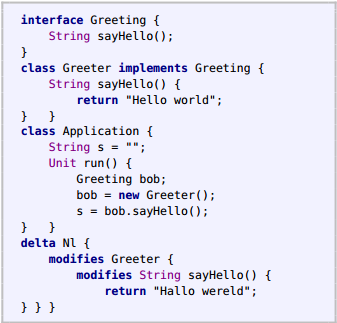
\includegraphics[width=0.6\textwidth]
        {img/delta-modeling-1.png}
    \caption{Delta Modelling pada ABS}
    \label{fig:clarkeDeltaExample}
\end{figure}
\vspace{-0.8cm}

\begin{center}
{\small Sumber gambar: \citep{clarke2012variability}}
\end{center}

Gambar \ref{fig:clarkeDeltaExample} diatas merupakan contoh penerapan \textit{delta modeling} pada bahasa pemodelan ABS. Seperti yang terlihat pada gambar tersebut, terdapat sebuah kode delta yang bernama \texttt{Nl}. kode delta \textit{Nl} tersebut melakukan sebuah modifikasi terhadap \textit{class} \texttt{Geater} dan \textit{method} \texttt{sayHello} dengan menggunakan kata kunci \texttt{modifies}. Kata kunci \texttt{modifies} merupakan kata kunci khusus pada ABS yang digunakan untuk memodifikasi \textit{interface, class} dan \textit{method}.\\

Selain kata kunci \texttt{modifies} seperti yang digunakan pada Gambar \ref{fig:clarkeDeltaExample} diatas, terdapat pula kata kunci kata kunci lain yang dapat digunakan dalam mendefinisikan kode delta pada ABS. Berikut ini adalah daftar kata kunci yang dapat digunakan berdasarkan dokumentasi ABS yang dibuat oleh \cite{absref2013}.

\begin{itemize}
    \item \texttt{modifies}: kata kunci ini digunakan untuk mendeklarasikan perubahan / modifikasi pada \textit{method, class, interface, module} dan \textit{data type} yang ada. sintaks yang digunakan adalah \texttt{modifies} diikuti dengan jenis dan nama elemen yang akan diubah seperti misalnya: \texttt{modifies class Greeter} yang ditujukan untuk melakukan modifikasi terhadap \textit{class} \texttt{Greeter}.
    \item \texttt{adds}: kata kunci ini digunakan untuk mendeklarasikan penambahan \textit{method, class, interface, module, import, export, field} dan \textit{data type} baru. sintaks yang digunakan adalah \texttt{adds} diikuti dengan jenis dan nama elemen yang akan ditambahkan pada sebuah \textit{interface, class, module} atau \textit{method}. Sebagai contoh, kita dapat menggunakan sintaks \texttt{adds interface MyInterface} untuk membuat sebuah interface baru dengan menggunakan \textit{delta modeling}.
    \item \texttt{removes}: kata kunci ini digunakan untuk menghapus \textit{method, class, interface} dan \textit{field} yang telah dibuat sebelumnya. sintaks yang digunakan adalah \texttt{removes} diikuti dengan jenis dan nama \textit{method, class, interface} atau \textit{field} seperti misalnya \texttt{removes String myField} yang digunakan untuk menghapus \textit{field variable} yang bernama \texttt{myField} pada sebuah \textit{class}.
\end{itemize}

Walaupun fitur \textit{delta modeling} sangat dinamis dalam melakukan perubahan, penambahan dan pengurangan elemen-elemen pada kode ABS, akan tetapi fitur ini memiliki beberapa keterbatasan yang diantaranya adalah:

\begin{enumerate}
    \item \textit{Class parameter} dan blok \texttt{init}: untuk saat ini kode delta belum dapat melakukan perubahan pada \textit{class parameter} dan blok init.
    \item Elemen fungsi pada program: kode delta hanya mendukung proses penambahan fungsi, penambahan dan pengubahan \textit{data type} dan \textit{type synonim} akan tetapi tidak mendukung proses penghapusan.
    \item Modul: untuk saat ini kode delta tidak dapat melakukan penambahan dan penghapusan modul.
    \item \texttt{Import} dan \texttt{Export}: kode delta hanya mendukung proses penambahan \textit{export} dan \texttt{import}.
    \item Blok utama: kode delta tidak mendukung perubahan pada blok utama program.
\end{enumerate}